\documentclass[review]{elsarticle}
\usepackage{graphicx}
\usepackage[svgnames]{xcolor}
\usepackage{algorithm}
\usepackage{graphicx}
\usepackage{graphicx}
\usepackage{algcompatible}
\usepackage{amsmath}
\usepackage{amssymb}
\usepackage{caption}
\usepackage{balance}
\usepackage{listings}
\usepackage{color}
\usepackage{float}
\usepackage[linewidth=1pt]{mdframed}
\definecolor{dkgreen}{rgb}{0,0.6,0}
\definecolor{gray}{rgb}{0.5,0.5,0.5}
\definecolor{mauve}{rgb}{0.58,0,0.82}
\usepackage{listings,chngcntr}
\lstset{frame=tb,
  language=Xml,
  aboveskip=3mm,
  belowskip=3mm,
  showstringspaces=false,
  columns=flexible,
  basicstyle={\small\ttfamily},
  numbers=none,
  numberstyle=\tiny\color{gray},
  keywordstyle=\color{blue},
  commentstyle=\color{dkgreen},
  stringstyle=\color{mauve},
  breaklines=true,
  breakatwhitespace=false,
  tabsize=1
}
\usepackage{amsmath}

\usepackage{lineno,hyperref}
\modulolinenumbers[5]

\journal{Journal of  Expert Systems with Applications}

%%%%%%%%%%%%%%%%%%%%%%%
%% Elsevier bibliography styles
%%%%%%%%%%%%%%%%%%%%%%%
%% To change the style, put a % in front of the second line of the current style and
%% remove the % from the second line of the style you would like to use.
%%%%%%%%%%%%%%%%%%%%%%%

%% Numbered
%\bibliographystyle{model1-num-names}

%% Numbered without titles
%\bibliographystyle{model1a-num-names}

%% Harvard
%\bibliographystyle{model2-names.bst}\biboptions{authoryear}

%% Vancouver numbered
%\usepackage{numcompress}\bibliographystyle{model3-num-names}

%% Vancouver name/year
%\usepackage{numcompress}\bibliographystyle{model4-names}\biboptions{authoryear}

%% APA style
\bibliographystyle{model5-names}\biboptions{authoryear}

%% AMA style
%\usepackage{numcompress}\bibliographystyle{model6-num-names}

%% `Elsevier LaTeX' style
\bibliographystyle{elsarticle-num}
%%%%%%%%%%%%%%%%%%%%%%%

\begin{document}

\begin{frontmatter}

\title{PAROT: Translating Natural Language  to SPARQL }


%% Group authors per affiliation:
\author{Peter Ochieng}
\address{Taita Taveta university,\\Nairobi,Kenya\\
onexpeters@gmail.com }
\fntext[myfootnote]{Since 1880.}



\begin{abstract}
This paper provides  a dependency based framework for converting natural language to SPARQL. We present a tool known as PAROT ( which echos answers from ontologies) which is able to handle user's  queries that contain compound sentences, negation, scalar adjectives and numbered list. PAROT employs  a number of dependency based heuristics to convert user's queries to user's triples. The  user's  triples are then processed by the lexicon  into ontology triples. It is these ontology triples that are used to construct SPARQL queries. From the experiments conducted, PAROT provides state of the art results.
\end{abstract}
\begin{keyword}
\texttt{SPARQL}\sep Natural Language Processing\sep Ontologies \sep Query
\end{keyword}

\end{frontmatter}

\section{Introduction}
In our bid to develop an ontology based chatbot,  we envision developing a tool that would allow users to  use their natural language (NL) and have a near natural conversation with a tool which fetches facts (answers) contained in an ontology based knowledge base (KB). This requires us to employ a plugin tool that translates the user's statements written in NL to  SPARQL query language \citep{Sparql12},  a W3C recommended language for querying ontologies. We experimented  with various NL to SPARQL tools  such as  AquaLog \citep{aqualog12}, CASIA@12  \citep{Casia12},  Querix \citep{Querix12}, AutoSPARQL \citep{autosparql12},   K-Extractor \citep{Kextractor12},    SPARK \citep{sparklis12} that currently exist in literature in order to select the best  tool. The best tool was to be selected  based on its precision and recall value ( i.e. its ability to fetch correct and all require answers).  However, we realized that despite the tools converting a number of  user's  queries to the correct SPARQL queries,  the tools' precision and recall values drastically dropped  for  queries  which contained:
\begin{enumerate}
\item Opposing scalar adjectives such as in the query
\textit{which is the \textbf{longest} and \textbf{ shortest} river that traverses Mississippi ?}, \citep{g2018} estimates that 12\% of the total errors in  queries generated by their gAnswer tool is due to the fact that it does not  support superlatives and comparatives in its implementation. This underscores the importance of handling scalar adjectives.
\item  Negation such as  \textit{which rivers do\textbf{ not} flow through Alaska ? or which river \textbf{neither} flows through Alaska nor Mississippi ?}.
\item Numbered list such as  \textit{list \textbf{five} rivers that flow through Alaska ?}
\item Compound sentences  \textit{which female actor played in Casablanca and is married to a writer born in Rome ?} . \citep{g2018} estimates that 9\% of the total errors in  queries generated by their gAnswer tool is due to the fact that it does not handle queries with unions or filters.
\end{enumerate} 
In addition to these weaknesses,  most of the state of  art tools use techniques that are not able to capture the entire vocabulary of the underlying knowledge base i.e. they don't generalize the entire knowledge base adequately. This affects the word disambiguation process hence reducing their precision and recall values.
\par This research addresses the above mentioned key challenges by introducing the following key concepts:
\begin{enumerate}
\item  Design a lexicon that that is able:
\begin{itemize}
\item To fully represent the vocabulary of the underlying knowledge base therefore helping in resolving word ambiguities that exist in the user's query.
\item To tag adjective entities in the knowledge base with their positive and negative scalars. Through this we are able to resolve the problem of opposing scalar adjectives when converting NL to SPARQL.
\end{itemize}
\item We develop  a number of high coverage  syntactic heuristics which can convert different scenarios of possible questions  to   correct SPARQL queries. 
\end{enumerate}
From the evaluation, the developed technique outperforms gAnswer \citep{g2018}, which was the top performing tool in QALD-9 challenge \citep{quad9}. This is due its  ability to effectively disambiguate  words and its high coverage of user questions.

\section{Literature Review}
In this section, we review state of the art applications that  converts NL to SPARQL as well as those that convert NL to SQL. We highlight the key techniques used by a tool and discuss whether it can handle the challenges discussed in section 1.
AquaLog \citep{aqualog12} is an ontology independent question answering system for the Semantic Web. It is composed of a linguistic component to map user query to query triples. It is these query triples that are further processed into an ontology compliant triples from where answers are derived. The linguistic component is composed of the GATE infrastructure  \citep{gate12} and resources to annotate the user query. The annotations in the user query include verbs, nouns, tokens etc. The component also employs JAPE grammars which expand annotations embedded by the GATE by  identifying terms, relations, question indicators (which/who/when, etc.) and patterns or types of questions.  AquaLog does not contain components  to deal with  scalar adjectives, numbered list and compound sentences. CASIA@12 \citep{Casia12} is a question answering system over linked data. After generating a number of possible phrase to semantic item mappings, it then uses Markov logic network (MLN) for disambiguation and finally form a SPARQL query. CASIA@12 does not handle scalar adjectives, negation, numbered list and compound sentences.  DEANNA \citep{Yahya2012} also translates a question  in NL into a structured query. The key element of DEANNA is the use integer linear program (ILP) to  solve the disambiguation of terms to semantic items. Querix \citep{Querix12} is a pattern matching ontology independent  natural language interface (NLI). Querix uses the Stanford parser to syntactically analyze the input query. From the syntax tree the query analyzer extracts the sequence of the key word categories such as Noun (N), Verb (V), Preposition (P), Wh-Word (Q), and Conjunction (C).  Based on the generated word categories a query skeleton is generated.  WordNet is used to supply all synonyms to the verbs and nouns in the query. It then matches the skeleton with triples in the ontology . In Querix  ambiguities are not resolved automatically  rather users are asked   for clarifications in a pop-up dialog menu window to disambiguate. Queries has a disadvantage that it only allows users  to write queries  starting with “which”, “what”, “how many”, “how much”, “give me” or “does” hence cannot handle questions starting with terms such as "List".  It also does not handle negation, scalar adjectives and extensively relies on WordNet which makes query generation process slow.   PANTO \citep{panto12} utilizes Stanford parser \citep{Klein2003} to generate a parse tree from the user submitted query. It then extracts nominal phrase constituents in the parse trees . The nominal phrases in the parse trees are extracted  as pairs to form an inter-mediate representation called QueryTriples.  It the utilizes the  knowledge in the ontology, to map QueryTriples to OntoTriples which are represented with entities in the ontology. Finally, together with targets and modifiers extracted from the parse trees, OntoTriples are interpreted as SPARQL. PANTO can handle conjunctions / disjunctions, negation, comparatives and superlatives. It however cannot handle opposing scalar adjectives and numbered list. AutoSPARQL \citep{autosparql12} uses  supervised machine learning to generate a SPARQL query based on positive i.e. resources which should be in the result set of the SPARQL query, and negative examples, i.e. resources which should not be in the result set of the query. The user can either start with a question as in other QA systems or by directly searching for a relevant resource. He or she can then select  an appropriate result, which becomes the first positive example. After that, he is asked a series of questions on whether a resource should also be contained in the result set. These questions are answered by  a ”yes“ or  a ”no“. This feedback allows the supervised learning method to gradually learn which query to generate. AutoSPARQL faces the challenge of  portability to a different Knowledge Base (KB) \citep{ontologysparql12}. The  effort of learning the positive and negative examples also increases drastically with the size of the KB \citep{ontologysparql12}. SPARK \citep{sparklis12} is another tool for  processing NL keyword to SPARQL.  Its  output is a ranked list of SPARQL queries.  Its key  steps include: term mapping, construction of the query graph and query ranking. Ranking of query applies a   probabilistic model based on the Bayesian Theorem. Its key challenge involves choosing an option out of the ranked query list since this requires  an expert in SPARQL who has  knowledge on the underlying KB  \citep{ontologysparql12}. Exploiting the recent success of deep learning, a number of studies introduce deep learning neural network based method to convert NL to structured query languages. Research in \citep{sema2019} applies a bidirectional long short term memory(LSTM) \citep{sema1997} network to convert NL to SPARQL. Bidirectional LSTM is employed  to capture the context of a word in relation to both the words before  and after  it. Their technique exploits the top key words in the submitted user question to extract candidate answers from the knowledge base. The words  are then linked to the correct answer tokens by learning their relatedness. WDAqua \citep{quad92018} generates SPARQL query from natural language  by employing rule-based  combinatorial approach to generate leveraging the semantics encoded in the underlying knowledge base.  Other state of the art tools for converting NL to SPARQL include  TeBaQA\citep{quad92018}, Elon\citep{quad92018} and QASystem\citep{quad92018}.  A complete review of NL to SPARQL tools is discussed in \citep{review1} , \citep{review2} and \citep{noma2018}. 
\par To convert NL to SQL, research in \citep{sema201},  employs a bidirectional LSTM to generate the best SQL query from a given NL. It applies encoder-decoder model proposed in \citep{sema2015}. In the decoder, the conditional probability distribution of the SQL token is predicted based on the previous combination of SQL token embeddings. They also incorporates human feedback to improve the learning process. Other studies that have exploited neural networks to convert NL to structured language include \citep{sema20p},\citep{Yu2018} and \citep{wera2018}. One major challenge with Neural Network based method is that they try to represent the whole knowledge base using a few training examples. This becomes a challenge when the model meets new vocabulary that  it had not seen in the training data hence affecting the prediction of neural network based. Table 1 gives a summary of  an evaluation of selected state of the art tools on whether they can handle negation, opposing scalar adjectives, compound sentences and the key disambiguation technique a tool applies.




\begin{center}
\begin{table}[H]
\caption{Evaluation of selected NL to structured language tools}
\resizebox{\textwidth}{!}{
\begin{tabular}{ |p{3.0cm}|p{2.0cm}|p{1.5cm}|p{1.7cm}|p{2.0cm}|p{2.6cm}| }
 \hline
 \textbf{Tool} &\textbf{Structured Language}& \textbf{Negation} & \textbf{Opposing Scalar adjectives}&\textbf{Compound sentences}&\textbf{Disambiguation Technique}\\\hline
 AquaLog \citep{autosparql12}&SPARQL&No&No&No&GATE infrastructure\\\hline 
CASIA@12 \citep{Casia12}&SPARQL&No&No&No&Markov Logic Network\\\hline
DEANNA \citep{Stoilos2005}&SPARQL&No&No&Yes&Integer linear programming\\\hline
Querix \citep{Querix12}&SPARQL&No&No&No&User\\\hline
PANTO \citep{panto12}&SPARQL&Yes&No&Yes&Query patterns\\\hline
AutoSPARQL \citep{autosparql12}&SPARQL& No&No&Yes&Machine learning\\\hline
 FREyA \citep{Freya12}&SPARQL&No&No&Yes&User\\\hline
  QuestIO&SPARQL&No&No&Yes&User\\\hline
  K-Extractor \citep{Kextractor12}&SPARQL&No&No&Yes&Ranking\\\hline
   SPARK \citep{sparklis12}&SPARQL&No&No&Yes&Ranking\\\hline
    SQLnet \citep{Nomas123}&SQL&yes&No&Yes&Neural Networt( LSTM)\\\hline
    DiaSQL \citep{wera2018}&SQL&yes&No&Yes&Neural Networt( LSTM)\\\hline
      SyntaxSQLNet\citep{Yu2018}&SQL&yes&No&Yes&Neural Networt( LSTM)\\\hline
      PAROT&SPARQL&yes&yes&Yes&Syctactic heuristic and Lexicon technique\\
      \hline
    
\end{tabular}}
\end{table}
\end{center}
\section{PAROT Architecture} 
\subsection{Step 1: Identifying targets.}
Given a user query submitted in natural language, the  first task is to identify targets  words from the query. A target (or projection) word  is a variable  that will be placed directly after SELECT key word in a SPARQL query. To help in  identifying  target words  in a  user submitted query, we  use a  typed dependency parser such as Stanford typed dependency parser \citep{Marneffe2015}. The dependency parser provides a simple description of grammatical relationships that exists between the words in the  user submitted query. To extract  the target words in the parsed query, we categorize the queries into two categories i.e.
\begin{itemize}
\item The  Wh (WRB, WP, WDT)  queries.
\item The non WH queries.
\end{itemize}
\subsubsection{ Targets in Wh based queries}
This category is composed of queries which start with \textit{Wh} (i.e. \textit{ what, when, where, who, whom, which, whose, why, and how)}. To identify target words in this category of queries, we apply two key set of rules in equation 1 and 2.

\begin{subequations}
\begin{align}
& \forall w_x,w_y.(nsubj(w_x,w_y)\implies Target(w_y)) \\
&\forall  w_x,w_y,w_z.(nsubj(w_x,w_y)\land conj(w_y,w_z)\implies Target(w_y)\land Target(w_z))
\end{align}
\end{subequations}
\begin{subequations}
\begin{align}
&\forall  w_x,w_y.(nsubjpass(w_x,w_y)\implies Target(w_y))\\
&\forall   w_x,w_y,w_z.(nsubjpass(w_x,w_y)\land conj(w_y,w_z)\implies Target(w_y)\land Target(w_z))
\end{align}
\end{subequations}
Here,  $dep(x,y)$ is a dependency that exists between words $x$ and $y$. The words of a sentence compose the constants of a domain over which the functions operate. The rules in  (1a) and (1b) apply  in a non relation query (see section 3.2.1 for definition of a relational and non-relational query). They basically identify the  nominal subjects in the user submitted query and flags them as targets. Equation (1a) applies for a query where there is no conjunct relation between the head subject of the query and any other nominal. For example, when a user submits a  query such as \textit{What is the area of the most populated state ?}, using  Stanford dependency parser, the dependency diagram in figure 1 is generated.
\begin{figure}[h]
	\centering
		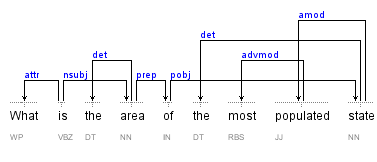
\includegraphics[scale=0.7,angle=0]{example2.png}
		\caption{Showing dependency }
	\label{fig:example2}
\end{figure}
The grounded version of formula (1a) is shown below.
\begin{equation*}
nsubj(is,area)\implies Target(area)
\end{equation*}
The dependency $nsubj(is,area)$ holds between the words \textit{is} and \textit{area}. Therefore, the nominal \textit{area}  is selected as the target of the query. If a user submits a query such as \textit{What is the area and population of the most populated state ?}, Stanford dependency viewer generates dependency shown in figure 2.
\begin{figure}[h]
	\centering
		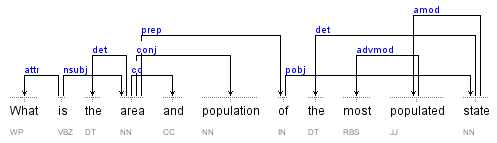
\includegraphics[scale=0.7,angle=0]{example1.png}
	\caption{Showing dependency }
	\label{fig:example1}
	\end{figure}
Since in this query the head subject \textit{area}  is  connected to another nominal by a coordinating conjunction \textit{``and'' },  the formula in equation (1b) is applied. 
\begin{equation*}
nsubj(is,area)\land conj(area,population)\implies Target(area)\land Target(population)
\end{equation*}
Both the nominals \textit{area} and \textit{population} are  selected as targets. This rule also captures scenarios where more than one nominal is connected to the head subject by a coordinating conjunction, such as \textit{and}, \textit{or} and ``,'' such as  \textit{What is the population, area and capital of the most populated state?}

The rules in equation (2a) and (2b) are  applicable in a relational based query. They  flag subjects word in a query by identifying the passive nominal subjects in the user submitted query. Equation (2a) is applicable where the head subject is not connected to any other nominal via a conjunction.  For example in the query \textit{ Which German actor was killed in a road crash ?}, the nominal \textit{actor} is selected as the target word.
\begin{equation*}
nsubjpass(killed,actor)\implies Target(actor)
\end{equation*}
  The rule in equation (2b)  captures scenarios where one or more  nominals  are connected to the head subject by a coordinating conjunction, such as \textit{and}, \textit{or} and ``,'' such as in the query \textit{Which German actor and musician were killed in a road crash?}. The nominals actor and musician are picked as target words.
 
\begin{equation*}
\begin{split}
nsubjpass(killed,actor)\land conj(actor,musician)\implies &Target(actor)\land \\&Target(musician)
\end{split}
\end{equation*}
\subsubsection{ Targets in non-WH  queries}
To  flag out target words in a non-Wh queries, we use the functions in equation 3 and 4. Equation (3a) and (3b) applies in a \textit{non-Wh} query that the direct object is not connected to a preposition such as \textit{ Give me all the rivers that traverse Mississippi}( see dependency diagram in figure 3). The rule in equation (3b) applies where the direct object is connected to one or more nouns  via a conjuction (e.g. \textit{Give me all rivers and lakes that traverse Mississippi})
\begin{subequations}
\begin{align}
\forall w_x,w_y.(dobj(w_x,w_y)\implies Target(w_y))\\
\forall   w_x,w_y,w_z.(dobj(w_x,w_y\land conj(w_y,w_z)\implies Target(w_y)\land Target(w_z))
\end{align}
\end{subequations}
\begin{figure}[h]
	\centering
		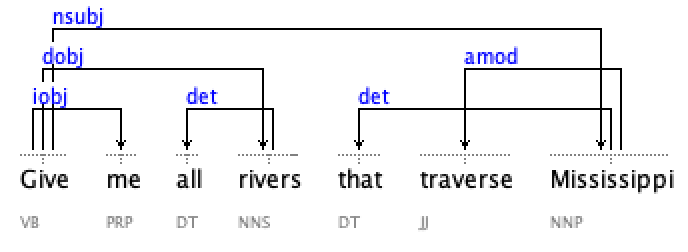
\includegraphics[scale=0.7,angle=0]{dobj.png}
	\caption{Showing dependency }
	\label{fig:example1}
	\end{figure}
\begin{subequations}
\begin{align}
\forall w_x,w_y.(pobj(w_x,w_y)\implies Target(w_y))\\
\forall   w_x,w_y,w_z.(pobj(w_x,w_y\land conj(w_y,w_z)\implies Target(w_y)\land Target(w_z))
\end{align}
\end{subequations}
Equation (4a) and (4b) applies in a non-Wh query that  the head  of a noun phrase folows a preposition.  Equation (4a) applies in  query such as \textit{In which country does the Nile start?}. Here,  the head noun \textit{country}  is not connected to any noun via a conjuction. Equation (4b) applies to a query where the head noun  is connected to one or more nouns via a conjuction such as in the query \textit{In which country and continent does the Nile start?}. The head  noun must be connected to a preposition.
\subsection{Step 2: Identifying user triple pattern}
SPARQL query is composed of a set of triple patterns known as graphs patterns. The graphs patterns  are placed directly after the WHERE key word or after the target variables in the SPARQL query. The triple patterns are of the form of $<subject> <predicate> <object>$ where the subject, predicate and object may be variables \citep{Sparql12}.  The idea therefore in this section is to process a user submitted query to identify potential triples that will be used to construct the SPARQL graphs. Triples identified from the user query are referred here as user triples. To identify user triples from the submitted query,  we categorize it into either:
\begin{enumerate}
\item Relational phrase based query.
\item Non-relational phrase based query.
\end{enumerate}

\subsubsection{ Identifying user  triple pattern in a relation based user query}
Relation based user query  is a query  which contains at least a relational phrase linking two nominals.  A relation phrase  can be a transitive verb (e.g. in the query  \textit{``which rivers traverse Alaska?'}', \textit{traverse} is a relational phrase) or intransitive verb followed with  prepositional complement ( e.g.  \textit{``which river flows through Alaska?'}', \textit{flows through} is a relational phrase). Therefore, a relational phrase linking two nominals may be a verb, a verb followed directly by a preposition  or a verb followed
by nouns, adjectives, or adverbs ending in a preposition  \citep{reverb12}.  

To identify user triples in a relation based  query, we apply Algorithm 1.
\begin{algorithm}
\begin{algorithmic}[1]
\caption{Extracting user triples from a relation based user query}
\STATEx \textbf{Input} \textit{Sentence S=($w_1,w_2\cdots w_n$)}.
\STATEx\textbf{Output} $UserTriples$.
\STATE Given a sentence $S=\left\{w_{1},w_{2},...,w_{n}\right\}$
\STATE Check if $S$ is compound i.e $CheckCompound(S)$. (equation 5)).
\IF {$CheckCompound(S)$=true.}
\STATE $Break(S)=(s_1(cc)s_2)$
\ELSE
\STATE $UserTriple=GenerateTriple(S)$.
\ENDIF
\STATE return $UserTriples$
\end{algorithmic}
\end{algorithm}
The algorithm accepts a user submitted query (sentence) which is composed of a number of words  as its input. It then evaluates if a sentence is compound  using the function \textit{checkCompound(S)}. The function $checkCompound(S)$  applies a number of  syntactic constraints to categorize a sentence as compound or not. The  syntactic constraints are shown in figure 4.  A compound sentence should be composed of the following sequence: 
\begin{enumerate}
\item A verb followed by a preposition followed by   a noun, conjuction and a verb (e.g. \textit{Which female actor \textbf{played in Casablanca and is married} to writer born in Rome})
\item verb followed by a noun followed by a conjuction and a noun(e.g. \textit{Which river \textbf{traverses Mississippi or Alaska}})
\item Noun followed by a conjuction followed by  a noun and a verb(e.g. \textit{Which \textbf{rivers and lakes traverse} Alaska}
\item An adverb, superlative followed by a conjuction followed by an adverb, superlative followed by a verb( e.g. \textit{Which is the\textbf{ least and most populated state } in America})\end{enumerate}

\begin{figure}[h]
	\centering
		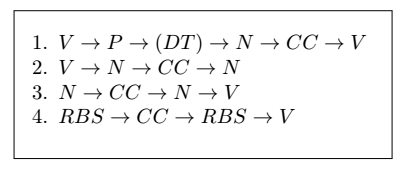
\includegraphics[scale=0.7,angle=0]{noma.png}
		\caption{POS tag patterns to flag compound  sentences in a relation based queries }
	\label{fig:example2}
\end{figure}

Using Stanford dependency parser, we translate the syntanctic constrains in figure 4 into a set of formulas shown in equation 5.
\begin{subequations}
\begin{align}
\begin{split}
&\forall w_e,w_h,w_i,w_j,w_k.(prep(w_e,w_h)\land pobj(w_h,w_i)\land cc(w_e,w_j)\land conj(w_e,w_k)\\
&\implies Compound(w_a,w_b,\cdots,w_n))
\end{split}\\
\begin{split}
&\forall   w_e,w_h,w_i,w_j.(dobj(w_e,w_h)\land cc(w_h,w_i)\land conj(w_h,w_j)\\
&\implies Compound(w_a,w_b,\cdots,w_n))
\end{split}\\
\begin{split}
&\forall  w_e,w_h,w_i,w_j.(nsubj(w_e,w_h)\land cc(w_h,w_i)\land conj(w_h,w_j)\\
&\implies Compound(w_a,w_b,\cdots,w_n)
\end{split}\\
\begin{split}
&\forall  w_e,w_h,w_i,w_j.(advmod(w_e,w_h)\land cc(w_h,w_i)\land conj(w_h,w_j)\\
&\implies Compound(w_a,w_b,\cdots,w_n)
\end{split}
\end{align}
\end{subequations}
Consider the sentence, \textit{S=which rivers traverse Mississipi or  Alaska}.  Applying  rule (5b),  the sentence is categorized as compound as shown below.
\begin{equation*}
\begin{split}
&dobj(traverse,Mississippi)\land cc(Mississippi,or)\land\\
&conj(Mississippi, Alaska)\implies Compound(S)
\end{split}
\end{equation*}
A sentence $S$ that is categorized as compound has to broken into two simple sentences $(s_1$ and $s_2)$. The sentences are  joined by a conjuction that was linking them in the user query i.e. $(s_1(cc)s_2)$. 
The function $Break(S)$ which is iterative applies  rule in equation 6 to extract two simple sentences from the compound sentence $S$.
\begin{equation}
Break(S)\equiv s_1 (cc) s_2
\end{equation}
where
\begin{subequations}
\begin{align}
s_1&=w_a,w_b,\cdots,w_i  \text{         } s_2=w_a,w_b,\cdots,w_{e-1},w_{j+1}\cdots w_n\\
s_1&=w_a,w_b,\cdots,w_h  \text{         }s_2=w_a,w_b,\cdots,w_{h-1},w_j\\
s_1&=w_a,\cdots,w_h,\cdots,w_{j+1}\cdots w_n \text{         } s_2=w_a,w_{i+1},\cdots,w_j,\cdots,w_n\\
s_1&=w_a,\cdots,w_h,w_{j+1}\cdots w_n \text{         } s_2=w_a,\cdots,w_{h-1}, w_j\cdots,w_n
\end{align}
\end{subequations}
The rule in equation (7a) applies to a compound sentence identified by the rule in equation (5a). Likewise, (7b) applies to (5b) ,(7c) to (5c) and (7d) applies to (5d).
 Here, we assume the last word of a sentence is $w_n$. Applying rule (7b),
the  compound sentence: \textit{S=which rivers traverse Mississipi and Alaska} is broken down into two simple sentences i.e.\\
$s_1$=\textit{Which rivers traverse Mississippi}.\\
$s_2$=\textit{Which rivers traverse Alaska}.\\
$cc=and$\\
Finally, the algorithm identifies triples through the function \textit{GenerateTriples}. For each simple sentence $s_i$,  \textit{GenerateTriple} function, identifies  user  triples in it by extracting  two subsequent head nouns and connects them using a relational phrase that links them. For instance, in $s_1$ above  we have the nouns \textit{rivers} and \textit{Mississippi} as  two subsequent head nouns and \textit{traverse} is the relational phrase linking them, therefore, \textit{GenerateTriple}  will generate  a single triple from  $s_1$ i.e. \textit\{rivers $traverse$ Mississippi\}. Likewise,  in $s_2$   a single user triple \textit\{rivers $traverse$ Alaska\}  will be generated. 
Once the user triples have been established, we generate all  triple arrangements that predict possible ways in which concepts in the user triples may be  modelled in the underlying ontology. For example,  the user  triple \textit{\{rivers $traverse$ Mississippi\}} predicts that the undelying ontology for instance has  modelled the concepts \textit{river} and \textit{Mississippi} as \textit{\{ river $:flows\_through$ Mississippi\}}. However, the undelying ontology may have modellled the concepts as \textit{\{ Mississippi :hasRiver river\}}. To capture both these possibilities, for each user triple we extract, we create a second one where the concepts in the subject and object position are  interchanged. Therefore, for the user triple  \textit{\{rivers $traverse$ Mississippi\}} we create another  \textit{\{Misssippi $traverse$ river\}} where the concepts \textit{Mississippi} and \textit{rivers} are interchanged. In this example we generate the following user triples.
$\textit{\{river traverse Mississippi OR  Mississippi traverse  river\}}$
$\textit{\{river traverse Alaska OR  Alaska traverse  river\}}$.
The correct arrangement of concepts as modelled in the ontology will be resolved by the lexicon.\\
Consider  the user query \textit{Which female actor played in Casablanca and is married to a writer born in Rome ?}, based on the rule in equation (5a), the query is marked as a compound sentence. The query is therefore   broken into two simple sentences i.e.\\
$s_1$= \textit{Which female actor played in Casablanca}\\
$s_2$=\textit{Which female actor is married to a writer born in Rome}.\\
$cc= And$\\
  When \textit{ GenerateTriple} function is applied to both $s_1$ and $s_2$, the following user triples are generated.\\
	$ GenerateTriple(s_1)$= \textit{\{actor $played\_in$ Casablanca}\}\\
	$GenerateTriple(s_2)$=\textit{\{actor $married\_to$  writer,	writer $born\_in$ Rome}\} \\
	
The user triples are then expanded to predict possible positions in the undelying ontologies.	
	 \textit{\{(actor $played\_in$ Casablanca, Casablanca $played\_in$ actor ) }\}\\
	\textit{\{(actor $married\_to$  writer, writer $married\_to$  actor)(writer $born\_in$ Rome, Rome $born\_in$ writer)}\} 
	
	
The final user triples generated from the query is shown in Listing 1.
\begin{lstlisting}[caption= Sample user triples]
{
(actor played_in Casablanca) OR (Casablanca played_in actor)  
                                      AND  
(actor married_to  writer)	OR (writer married_to  actor)
(writer born_in Rome) or (Rome born_in writer)
}
\end{lstlisting}
The correct position of the concepts as modelled in the undelying ontology will be resolved by the lexicon as discussed in section 3.5.
There are two special cases  where  $GenerateTriple$  applies  the rules in equation 8. The rules basically apply in scenarios where it is not explicit which nouns a verb is linking. The rules are applied;
\begin{enumerate}
\item When a query starts with \textit{Who} e.g \textit{Who killed Ceasar ?}
\item  When a query contains a verb that does not lie between any two nouns ( i.e. when a verb is at the end of a sentence such as in the query\textit{ In which continent does the Nile traverse ?}.
\end{enumerate}
Rule (8a) applies for the first scenario while (8b) for the second.
\begin{subequations}
\begin{align}
\begin{split}
&\forall  w_e,w_h,w_i.(nsubj(w_e,w_h)\land dobj(w_e,w_i)
\implies Triple( ?w_h,w_e,w_i))\lor \\
&Triple( w_i,w_e,?w_h))
\end{split}
\end{align}
\begin{align}
\begin{split}
&\forall  w_e,w_h,w_i,w_j.(pobj(w_e,w_h)\land prep(w_j,w_e)\land nsubj(w_j,w_i)\\
&\implies Triple( w_i,w_j,w_h)\lor Triple( w_h,w_j,w_i)
\end{split}
\end{align}
\end{subequations}

\begin{figure}[h]
	\centering
		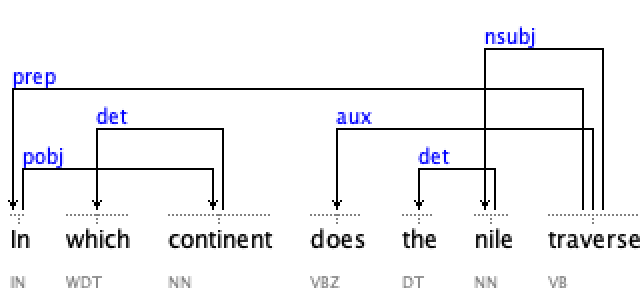
\includegraphics[scale=0.7,angle=0]{nile.png}
		\caption{Showing dependency }
	\label{fig:example2}
\end{figure}
Consider the query \textit{Who killed Ceasar ?}, applying the rule in equation (8a),
\begin{equation*}
\begin{split}
&nsubj(killed,who)\land dobj(killed,Ceasar)
\implies Triple( ?who,killed,Ceasar)\lor\\
&Triple( Ceaser,killed,?who)
\end{split}
\end{equation*}
the user triple \textit{\{?who killed Ceasar\}} or \textit{\{Ceaser  killed ?Who\}}  is generated. Again consider the user query  \textit{ In which continent does the Nile traverse ?}. The dependency diagram is shown in figure 5. Applying the rule in equation (8b),
\begin{equation*}
\begin{split}
&pobj(In,continent)\land prep(traverse,In)\land nsubj(traverse,Nile)\\
&\implies Triple( Nile,traverse,continent)\lor Triple( Continent,traverse,Nile)
\end{split}
\end{equation*}
 
\begin{lstlisting}[caption= Sample user triples]
{
(nile traverse continent)   or (continent traverse nile)
         
}

\end{lstlisting}
\subsubsection{ Identifying user query triple pattern in non-relation based user query}
A non-relational query is a query (sentence)  which has no relational phrase  linking  any of its nominals. For instance,  the sentence  \textit{What is the area of the most populated state?} is a non-relation based query. To identify triples that exist in this category of queries, we use Algorithm 2.
\begin{algorithm}[H]
\caption{Triple extraction Algorithm in a non-relational query}
\begin{algorithmic}[1]
\STATEx \textbf{Input} $Sentence S=(w_1,w_2\cdots w_n)$.
\STATEx \textbf{Output} $UserTriples$.
\STATE Given a sentence $S=(\left\{w_{1},w_{2},...,w_{n}\right\})$
\STATE Check if it is compound i.e $CheckCompound2$(S) (equation 9,10 or 11)).
\IF {$CheckCompound2(S)==true$}
\STATE $(s_1,s_2)=Break2(S)$
\ELSE
\STATE $UserTriples=GenerateTriple2$(S).
\ENDIF
\STATE return $UserTriples$
\end{algorithmic}
\end{algorithm}
The function $CheckCompound2$ establishes whether a non-relation query  is compound or not based on two key rules developed. The  rules  in equation 9 and 10 applies for \textit{Wh}  and \textit{non-Wh}  based queries respectively. The rule in equation 11 applies for  a a non relational query that contains the pattern $JSS\rightarrow CC\rightarrow JJS\rightarrow N$ i.e. an adjective, superlative followed by a conjuction followed by an adjective, superlative followed by a noun( e.g. \textit{Which is the\textbf{ longest and shortest river} in America}).
\begin{equation}
\begin{split}
 &\forall  w_d,w_f,w_g,w_k.(nsubj(w_d,w_f)\land cc(w_f,w_g)\land conj(w_f,w_k)\\
 &\implies Compound(w_a,w_b,\cdots,w_n)
 \end{split}
\end{equation}
\begin{equation}
\begin{split}
 &\forall  w_d,w_f,w_g,w_k.(dobj(w_d,w_f)\land cc(w_f,w_g)\land conj(w_f,w_k)\\
 &\implies Compound(w_a,w_b,\cdots,w_n)
 \end{split}
\end{equation}
\begin{equation}
\begin{split}
&\forall  w_e,w_h,w_i,w_j.(amod(w_e,w_h)\land cc(w_h,w_i)\land conj(w_h,w_j)\\
&\implies Compound(w_a,w_b,\cdots,w_n)
\end{split}
\end{equation}
A compound sentence is broken into two  simple sentences,   $s_1, s_2$ as shown in the rule in equation 12. where
\begin{equation}
Break2(S)\equiv s_1(cc)s_2
\end{equation}
Where in a compound sentence identified by rule 9 and 10\\
$s_1=w_a,w_b,\cdots ,w_f,w_{k+1},\cdots,w_n$\\
$s_2=w_a,w_b,\cdots,w_{f-1},w_{g+1}\cdots w_n$\\
while in a compound sentence identified by rule 11\\
$s_1=w_a,\cdots,w_h,w_{j+1}\cdots w_n$ \\
$s_2=w_a,\cdots,w_{h-1}, w_j\cdots,w_n$\\
Consider the user query  \textit{S=What is the population and area of the most populated state ?}. The dependency diagram is shown in figure 2.  Applying equation 10,
\begin{equation*}
\begin{split}
 &nsubj(is,population)\land cc(population, and)\land conj(population,area)\\
 &\implies Compound(S)
 \end{split}
 \end{equation*}
Since the sentence is compound, the $ Break2(S)$ function is applied  to break it into two simple sentences $s_1$ and $s_2$ i.e.\\
$s_1$=\textit{What is the population of the most populated state}\\
$cc$= And\\
$S_2$=\textit{What is the area of the most populated state}\\
Finally, user triples  are identified through the function $GenerateTriples2$.  To identify triples, $GenerateTriples2$  exploits the presence of;
\begin{enumerate}
\item Preposition (\textit{father of Tom or mountain in Germany}).
\item Genitive's construction ( Tom's father).
\end{enumerate} 
The preposition \textit{ ``of"} signals that a given noun posess a specified property e.g. in the query \textit{What is the \textbf{area of} the most populated state} suggests that the noun
\textit{state} has a property \textit{ area}. The preposition \textit{in} is a signal that  a given object belong to a noun e.g. \textit{What is the highest \textbf{mountain in} Germany} depicts that Germany has an object of the type \textit{mountain}. Therefore based on the type of preposition used, $GenerateTriples2$ uses two key set of rules to extract triples from a user submitted query. When using a preposition to extract triples, the  general syntactic constraint  in non-relation based query is \textit{$N \rightarrow  IN \rightarrow (A^{*})\rightarrow N$} i.e. a noun followed by a preposition followed by a noun. Sometimes a determinant and an adjective may exists as depicted by $A^{*}$.
The rules in equations 13  apply for a query where \textit{of} preposition is used.  Equation (13a) and (13b) are exploited for  \textit{Wh}   and  \textit{non-Wh} based queries respectively.
\begin{subequations}
\begin{align}
\begin{split}
 &\forall   w_u,w_x,w_y,w_z.(nsubj(w_u,w_x)\land prep(w_x,w_y)\land pobj(w_y,w_z)\land(w_y= ``of")\\
 &\implies Triple(w_z,(w_x\_w_y), ?k))
\end{split}\\
\begin{split}
 &\forall   w_u,w_x,w_y,w_z.(dobj(w_u,w_x)\land prep(w_x,w_y)\land pobj(w_y,w_z)\land(w_y=``of")\\
 &\implies Triple(w_z,(w_x\_w_y), ?k))\\
\end{split}
\end{align}
\end{subequations}
Hence, applying $GenerateTriples2$ (rule (13a)) to $s_1$ and $s_2$\\
\begin{equation*}
\begin{split}
 &(nsubj(is, population)\land prep(population,of)\land pobj(of,state)\land(of= ``of")\\
 &\implies Triple(state,(population\_of), ?k))
 \end{split}
\end{equation*}
\begin{equation*}
\begin{split}
 &(nsubj(is, area)\land prep(area,of)\land pobj(of,state)\land(of= ``of")\\
 &\implies Triple(state,(area\_of), ?k))
 \end{split}
\end{equation*}
$GenerateTriples2(s_1)$=\{\textit{State $population\_of$ ?x\}}\\
$GenerateTriples2(s_2)$=\{\textit{State $area\_of$ ?x\}}\\

$UserTriples$=\{\textit{State $population\_of$ ?x AND State $area\_of$ ?y\}}
\begin{lstlisting}[caption= User triples]
{
State population_of ?x
          AND  
State area_of ?y
}
\end{lstlisting}
For a case where the \textit{in} preposition is used, equation (14a) and (14b) applies for \textit{Wh} and \textit{non-Wh} based questions respectively.
\begin{subequations}
\begin{align}
\begin{split}
  &\forall   w_u,w_x,w_y,w_z.(nsubj(w_u,w_x)\land prep(w_x,w_y)\land pobj(w_y,w_z)\land(w_y = ``in")\\
 &\implies Triple(w_z,?k, w_x ))\lor Triple(w_x,?k, w_z))
\end{split}\\
\begin{split}
 &\forall   w_u,w_x,w_y,w_z.(dobj(w_u,w_x)\land prep(w_x,w_y)\land pobj(w_y,w_z)\land(in = ``in")\\
 &\implies Triple(w_z,?k,w_x )\lor Triple(w_x,?k, w_z))
\end{split}
\end{align}
\end{subequations}
Consider the user query \textit{Which is the highest mountain in Germany ?}, applying the rule in equation (15a),
\begin{equation*}
\begin{split}
  &nsubj(is,mountain)\land prep(mountain,in)\land pobj(in,Germany)\land(w_y = ``in")\\
 &\implies Triple(Germany,?k, mountain )\lor Triple(mountain ,?k, Germany))
\end{split}
\end{equation*}
The user triple\textit{\{Germany ?k Mountain\} or \{Mountain ?k Germany\}} is extracted.\\
Here,  we try to  preempt all the possible  the arrangements of concepts in the underlying ontology. The term $Germany$ could be modeled in the ontology to occupy the subject position such as in the triple \textit{\{Germany :hasMountain Adelegg\}} or it can be modeled to occupy the object position such as  \textit{\{Adelegg :belongTo Germany\}}. The exact triple to be selected will be determined by the lexicon.
When it comes to  genitive's complement the rule in equation 15 is applied. The syntactic constraint applied is \textit{$ N\rightarrow POS\rightarrow N$} i.e. it involves  two nouns, the head and the dependent (or modifier noun)(e.g German's flag). The dependent noun modifies the head by expressing some property of it. The rule in (15a) is applicable in a \textit{non-Wh} query while (15b) applies in a  \textit{Wh} based queries.
\begin{subequations}
\begin{align}
\begin{split}
    &w_u,w_x,w_y,w_z.(dobj(w_u,w_x)\land poss(w_x,w_y)\land possessive(w_y,w_z)\\
 &\implies Triple(w_y,?k, w_x ))\lor Triple(w_x,?k, w_y))
\end{split}\\
\begin{split}
   &w_u,w_x,w_y,w_z.(nsubj(w_u,w_x)\land poss(w_x,w_y)\land possessive(w_y,w_z)\\
 &\implies Triple(w_y,?k, w_x ))\lor Triple(w_x,?k, w_y))
\end{split}
\end{align}
\end{subequations}
Consider the query \textit{ What is Angela's birth name?}( see dependency in figure 6), applying the rule in equation (15b),
\begin{equation*}
\begin{split}
 &nsubj(is,name)\land poss(name,Markel)\land possessive(Markel,'s)\\
 &\implies Triple(Markel,?k, name )\lor Triple(name,?k, Markel))
 \end{split}
\end{equation*}
 The triple \textit{\{Markel, ?k name\}$\lor$ \{name,?k, Markel\}} is generated.
 \begin{figure}[h]
	\centering
		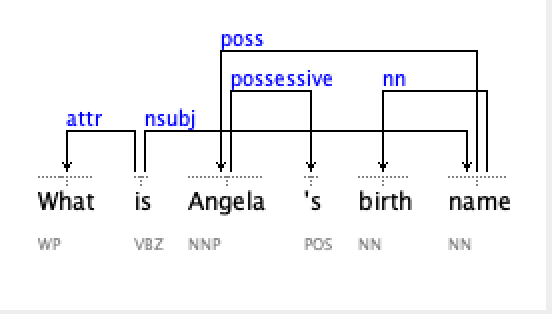
\includegraphics[scale=0.7,angle=0]{angel.png}
		\caption{Dependency diagram }
	\label{fig:example2}
\end{figure}
\subsection{Step 3: Handling adjectives}
To handle adjectives, we categorize them into two groups
\begin{enumerate}
\item Scalar adjectives.
\item Non-scalar adjectives.
\end{enumerate}
\subsubsection{Scalar adjectives}
Scalar adjectives are those which communicate the  idea of scale. In OWL ontologies, scalar adjectives can be mapped to an owl:DatatypeProperty. To flag out scalar adjectives, we use two two key syntactic constraints
\begin{figure}[H]	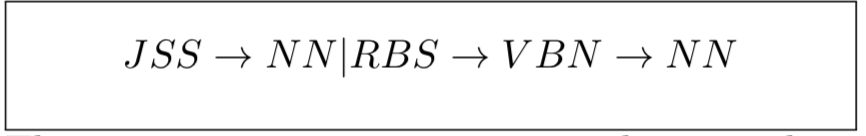
\includegraphics[scale=0.5,angle=0]{adjectiveSA.png}
		\caption{POS tag patterns for scalar adjective  }
	\label{fig:example2}
\end{figure}The syntactic constraint requires that a scalar adjective
matches any of the the POS tag pattern shown in figure 7. The pattern limits a scalar adjective to be
\begin{enumerate}
\item An  adjective, superlative followed by a noun ( e.g., longest river).
\item An adverb, superlative followed by a verb followed by a noun (e.g., most populated state)
\end{enumerate}
A scalar adjective is a signal that a given noun posses a  property  indicated by the adjective. For example the combination \textit{longest river} is an indication that the noun river has a property \textit{length}.
We therefore translate the syntactic contraints in figure 7 to  the rules in equation 16 and 17. The rules are used  to create triples from a query that contains a scalar adjective.
\begin{equation}
 \forall  w_u,w_x,w_y.(amod(w_x,w_u)\land (w_u\equiv JJS)\implies Triple(w_x,root(w_u), ?k))
\end{equation}
\begin{equation}
 \forall   w_u,w_x,w_y.(advmod(w_x,w_u)\land amod(w_y,w_x)\implies Triple(w_y,root(w_x), ?k))
\end{equation}
Consider the query \textit{Which is the longest river in America ?}. Applying the rule in equation 16, the  user triple in Listing 4 is generated.\\
$amod(river,longest)\land (longest\equiv JJS)\implies Triple(river,root(longest), ?k))$\\
\begin{lstlisting}[caption= User triples]
{
River long ?x
}
\end{lstlisting}
Consider the query \textit{Which is the most populated state in America ?}. Applying the rule in equation 18, the user  triple in Listing 5 is generated.\\
\begin{equation*}
\begin{split}
&advmod(populated,most)\land amod(state, populated)\\
& \implies Triple(state,root(populated), ?k))
\end{split}
\end{equation*}
\begin{lstlisting}[caption= User triples]
{
State population ?x
}
\end{lstlisting}
\subsubsection{Non-scalar adjectives}
These are adjectives that do not communicate the idea of scale. For a non-scalar adjective, we restrict that a syntactic constraint must match the POS tag patterns shown in figure 8. The pattern limits a non-scalar adjective to be an adjective followed directly by another adjective then a noun (e.g. female Russian astronaut) or an adjective followed directly by a noun (e.g., German chemist). 
\begin{figure}[H]	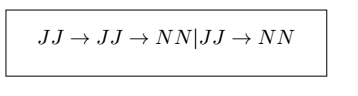
\includegraphics[scale=1.0,angle=0]{nons.png}
		\caption{POS tag patterns for non-scalar adjective  }
	\label{fig:example2}
\end{figure}
The POS tag pattern is translated into the rule in equation 18 and 19 respectively. The functions try to preempt all the possible modelling of the  concepts' positions in the  underlying ontology. Consider the statement \textit{German  fighter}. An ontology can model this in two possible ways i.e \textit{fighter :hasNationality German} or \textit{Germany :hasFighter  fighter} hence the word \textit{fighter} can be modelled in the subject or object position. When extracting the user triples in equation 18 and 19, we extract the two possibilities.
\begin{equation}
\begin{split}
 &\forall w_u,w_x,w_y.(amod(w_x,w_u)\land amod(w_x,w_y)\\
 &\implies (Triple(w_x,?k, w_u)\land Triple(w_x,?k, w_y))\lor\\ &(Triple(w_u,?k, w_x)\land Triple(w_y,?k, w_x))
 \end{split}
\end{equation}
\begin{equation}
 \forall  w_u,w_x.(amod(w_x,w_u)\implies Triple(w_x,?k, w_u))\lor Triple(w_u,?k, w_x))
\end{equation}
Applying the rule in equation 19  to the user  query  \textit{Which German chemist won the Nobel prize ?}\\
$amod(Chemist, German)\implies$ \textit{Triple(Chemist ?k German)}$\lor$ \textit{Triple(German ?k Chemist)} \\
Likewise applying the rule in equation 18 to the user  query  \textit{Which female German chemist won the Nobel prize}\\
\begin{equation*}
\begin{split}
&amod(Chemist, German)\land amod(female, German)\implies\\
&\textit{Triple(Chemist ?k German)} \land \textit{Triple(Chemist ?k female)}\lor\\
&\textit{Triple(German ?k Chemist)} \land \textit{Triple(female ?k German)}
\end{split}
\end{equation*}
The user triples of a user query generated based on adjectives are added to the existing user triples generated in the previous step.  For example in the query \textit{Which female German chemist won the Nobel prize ?},  since it is a relation based query,  it is first processed  based on the discussion in 3.3.1,  the $GenerateTriple(s)$ will extract the triples \textit{\{(Chemist won Nobel)or (Nobel won Chemist)\}}. Adding this to the triple generated based on adjective, the final user triples for the query is shown  in Listing 6.

\begin{lstlisting}[caption= User triples]
{
(Chemist  ?k German) OR (German ?k Chemist)
(Chemist won Nobel) OR  (Nobel won Chemist)
}
\end{lstlisting}
\subsection{Lexicon}
The words in user triples need to be mapped to the entities in the underlying ontology i.e. the user triples need to speak the language of the ontology. For instance, the terms in the user triple
\textit{\{State population\_of ?x\}}  in Listing 3  need to be mapped to the terms  \textit{\{State :hasPopulation ?x\}} in the ontology in  Listing 7.  For this purpose  a lexicon is developed. 

\begin{lstlisting}[caption= Sample ontology]
 <rdf:RDF xmlns:rdf="http://www.w3.org/1999/02/22-rdf-syntax-ns#"
 xmlns:rdfs="http://www.w3.org/2000/01/rdf-schema#"
xmlns:owl="http://www.w3.org/2002/07/owl#"
 xml:geo="http://www.geo.net/geography/geo.owl">
 <owl:ObjectProperty rdf:ID="flow_through">
 <rdfs:domain rdf:resource="#River"/>
 <rdfs:range  rdf:resource="#State"/>
 </owl:ObjectProperty>
 <owl:Class rdf:ID="River">
 <rdfs:subClassOf rdf:resource="#WaterBody"/>
 <rdfs:subClassOf>
<owl:Restriction>
<owl:onProperty  rdf:resource="#hasPopulation"/>
<owl:allValuesFrom rdf:datatype="http://www.w3.org/2001/XMLSchema#positiveInteger"/>
</owl:Restriction>
</rdfs:subClassOf>
 </owl:Class>
 <owl:Class rdf:ID="State">
 <rdfs:subClassOf rdf:resource="#Counties"/>
 </owl:Class>
 <River  rdf:ID="Mississippi_river">
 <owl:flow_through rdf:resource="#Mississippi_state"/>
 </River>
 <State  rdf:ID="Mississippi_state">
 <owl:hasPopulation rdf:datatype="http://www.w3.org/2001/XMLSchema#positiveInteger">50000000</owl:hasPopulation>
 </State>
 <State  rdf:ID="Texas">
 <owl:hasPopulation rdf:datatype="http://www.w3.org/2001/XMLSchema#positiveInteger">298465775</owl:hasPopulation>
 </State>
 <State  rdf:ID="Georgia">
 <owl:hasPopulation rdf:datatype="http://www.w3.org/2001/XMLSchema#positiveInteger">4657985</owl:hasPopulation>
 </State>
 <owl:DataProperty rdf:ID="hasPopulation">
 <rdfs:domain rdf:resource="#State"/>
 <rdfs:range  rdf:resource="http://www.w3.org/2001/XMLSchema#positiveInteger"/>
 </owl:ObjectProperty>
</rdf:RDF>
\end{lstlisting}
The lexicon helps in mapping user terms to the entities in the ontology. A lexicon records information specific to individual entities ( classes, predicates and individuals) contained in the ontology. We believe that a good lexicon should be rich enough to :
\begin{enumerate}
\item Disambiguate words such as Mississippi river and Mississippi state.
\item Identify positive and negative scalar adjectives in a user triple.
\item Map words in a way that minimizes the search space.
\item Resolve the exact position of a concept as modelled in the underlying ontology.
\end{enumerate}
To develop this kind of a lexicon, we adopted lemon (Lexical Model for Ontologies) \citep{john2011} which is a model for lexicons that are machine readable. It allows information to be represented relative to the underlying ontology. Lemon was a natural  choice  since it is RDF based and uses the principles of Linked Data. It can  also be extended  easily to capture the information  needed.  To reduce the work of generating the lexicon manually,  we adopted the technique proposed in \citep{walter2013}.  We exploited the technique to generate the lexicon in lemon model  semi-automatically.  We designed the lexicon such that it preserved  the structure of the underlying ontology. For each lexical entry in the lexicon we specify the following information:

\begin{lstlisting}[caption= Sample lexicon created from the ontology in Listing 7,
    basicstyle=\footnotesize
]
<?xml version="1.0"?>
:state a lemon:LexicalEntry ;
lexinfo:partOfSpeech lexinfo:noun ;
lexinfo:type lexinfo: class ;
lexinfo:OntotripleCategory lexinfo: subject ;
lexinfo:AsscociatedPredicate lexinfo: hasPopulation ;
lexinfo:AsscociatedObject lexinfo: positiveInteger ;
lexinfo:positive lexinfo: most populated ;
lexinfo:positive lexinfo: most inhabited ;
lexinfo:negative lexinfo: least populated ;
lexinfo:negative lexinfo: least inhabited ;
 lemon:canonicalForm [ lemon:writtenRep "state"@en];
  lemon:sense [ lemon:reference
<http://dbpedia.org/ontology/state >].

:river a lemon:LexicalEntry ;
lexinfo:partOfSpeech lexinfo:noun ;
lexinfo:type lexinfo: class ;
lexinfo:OntotripleCategory lexinfo: subject ;
lexinfo:AsscociatedPredicate lexinfo: flows_through ;
lexinfo:AsscociatedObject lexinfo: state ;
 lemon:canonicalForm [ lemon:writtenRep "river"@en];
  lemon:sense [ lemon:reference
<http://dbpedia.org/ontology/river >].
\end{lstlisting}

\begin{enumerate}
\item \textit{  LexicalEntry }. This  is a  given ontology entity (class, property or individual) extracted  from the underlying ontology e.g. the entity \textit{River} in Listing 7.
\item \textit{ partOfSpeech }. This entry specifies  the  part of speech to which the word in the  \textit{LexicalEntry} belongs to.
\item \textit{ canonicalForm}.  This is  the lemma of the word in the \textit{ LexicalEntry}. To extract a canonical for of a verb, its  lemma is  its  infinitive form or its present tense (e.g. the canonical form of the verb married  is  marry) .  The  canonical form a noun is the noun's singular form ( e.g. the canonical form of the noun Rivers is  River). For the  adjectives it is the positive (i.e., non-negative, non-graded) form (e.g. high).
\item \textit{ type}. This is the \textit{rdf:type} of the \textit{LexicalEntry}.
\item \textit{ OntotripleCategory}. This indicates the position of the \textit{ LexicalEntry} in the ontology triple i.e. is it a subject, predicate or an object. If the \textit{ LexicalEntry} is a subject, then the its associated   \textit{ predicate} and \textit{ object} must be specified. Likewise,  if it is an object then its asscotiated  \textit{subject} and \textit{ predicate} should be indicated  and finally if the lexical item is predicate then  its associated \textit{ subject} and \textit{ object} should be indicated.
\item \textit{ positive}  and \textit{negative} entries. These entries  are included for a \textit{ LexicalEntry } which is a domain of a \textit{owl:DatatypeProperty} where the asscociated  range is a non-negative integer.  They give the positive and negative scalar adjectives associated with the \textit{ LexicalEntry }. For example in Listing 7, the entity $State$  is the domain of the property $hasPopulation$ and its range is a non-negative integer. Therefore its positive and negative scalar adjectives must be indicated.  The  positive scalar adjectives asscociated with the word $State$ w are  \textit{Most Populated} and \textit{Most Inhabited} while negative include \textit{Least populated} and \textit{Least Inhabited}. This entries are helpful when processing sentences that contain scalar adjectives such as  \textit{"Which is the most populated state in USA}, the term \textit{most populated} will be mapped to a  positive scalar adjective in the lexicon.
\end{enumerate}
A sample lexicon extracted from the ontology in listing 7 is shown in Listing 8.  
\subsection{Step 4: Converting user triples to ontology triples}
The user triples need to be converted to ontology triples using the lexicon. To do this, terms in the user triples need to be mapped to the terms in the underlying ontology. To map a user triple to an ontology triple, the position a term occupies in the user triple should match the position of the term it is mapped to in the ontology triple i.e. a term in the user triple that occupies the subject position must be mapped to a term in the ontology triple that occupies subject position. By doing this, we narrow the search space hence reducing the mapping time significantly.  A user triple can be in any of this forms
\begin{enumerate}
\item  $ (\langle x\rangle\langle y\rangle\langle z\rangle)$
\item  $ (\langle ?x\rangle\langle y\rangle\langle z\rangle)$
\item  $ (\langle x\rangle\langle ? y\rangle\langle z\rangle)$
\item  $ (\langle x\rangle\langle y\rangle\langle ?z\rangle)$
\end{enumerate}
Given a user triple in the form  $ (\langle x\rangle\langle y\rangle\langle z\rangle)$ or   $( \langle z\rangle\langle y\rangle\langle x\rangle) $
 e.g. \textit{(actor $played\_in$ Casablanca)} or \textit{(Casablanca $played\_in$ actor ) }   the lexicon has to perform two key tasks.
\begin{enumerate}
\item When a user triple presents two options, it should select the correct triple that reflects the modelling in the underlying ontology.
\item Map user terms to ontology terms( i.e. bridge the gap between user terms and ontology terms).
\end{enumerate}
Using string metric \citep{Stoilos2005} and background knowlege Wordnet, the user entity 
$ x$ from the user triple  $ (\langle x\rangle\langle y\rangle\langle z\rangle)$ or   $( \langle z\rangle\langle y\rangle\langle x\rangle) $ is mapped to the lexical entry $x\_lexicon$ in the lexicon. Once the term $ x$  is mapped to a term $x\_lexicon$ in the lexicon, the lexicon is queried  to fetch all lexical entries that contain the term $x\_lexicon$. We then select all 
$x\_lexicon$ where $<ontotripleCategory>$ is the subject i.e. we  select all $x\_lexicon$ that occupy the subject position. We then map the  $<object>$ of $x\_lexicon$ to the $<object>$ of $ x$ in the user triple i.e. $<object>$ of $x\_lexicon$ is compared with  $\langle z\rangle$. If they match then the terms of the user triple $\langle x\rangle\langle y\rangle\langle z\rangle)$ are mapped position by position to the lexicon terms $\langle x\_lexicon\rangle\langle y\_lexicon\rangle\langle z\_lexicon\rangle)$. The second option $( \langle z\rangle\langle y\rangle\langle x\rangle) $ is hence dropped. If they don't match  the lexicon is queried to fetch $x\_lexicon$  that occupies the $<object>$  position.  We then map the  $<subject>$ of $x\_lexicon$ to subject  in the user triple i.e. $<subject>$ of $x\_lexicon$ is compared with  $\langle z\rangle$. If they match  then the terms of the user triple $\langle z\rangle\langle y\rangle\langle x\rangle)$ are mapped position by position to the lexicon terms $\langle z\_lexicon\rangle\langle y\_lexicon\rangle\langle x\_lexicon\rangle)$. The first option $( \langle x\rangle\langle y\rangle\langle z\rangle $ is hence dropped. The same technique is applied for the various forms of user triples generated.
\section{Query Construction}
After converting user triples into   ontology triples, the next stage is to generate a SPARQL query. The general syntax of the SPARQL query is shown in Listing 9.
\begin{lstlisting}[caption= SPARQL query structure]
SELECT ?target1 ?target2 ...?targetn
WHERE {
Ontology triples 
} Modifiers
\end{lstlisting}
The targets are the words identified in step 1 (section 3.1). For instance, consider the sentence \textit{what is the area and population of the most populated state}, from the rule in equation (1b), the words \textit{area} and \textit{population} will be identified as the targets.
Therefore the intial SPARQL query generated will be
\begin{lstlisting}
SELECT ?area ?population
{
}
\end{lstlisting}
After identifying targets, the next step is to identify the user triples as discussed in step 2 (section 3.2). In the sentence  \textit{what is the area and population of the most populated state}, since this query is a non-relation based query, it will be processed based on the discussion in section 3.2.2. The user triple is shown in Listing 3.  After generating user triples, the next step is to convert the user triples into ontology triples by the use of the lexicon as discussed in section 3.5.  The triples that will be generated in our running example will be:
\begin{lstlisting}[caption= SPARQL construction]
SELECT ?area ?population
{
State :hasPopulation ?population.
              AND
State :hasArea ?area.
} 
\end{lstlisting}
For each unique noun \textit{X} that appears in the subject position of the ontology  triple, we add the triple $<?x>$ $<rdf:type>$ $<X>$ and replace the all the  subsequent noun  \textit{X}  in the ontology triples with $<?x>$. Therefore, the triple ontology triples in Listing 10 is expanded to Listing 11.
\begin{lstlisting}[caption= SPARQL construction]
SELECT ?area ?population
{
?state rdf:type :State
?state :hasPopulation ?population.
              AND
?state :hasArea ?area.
} 
\end{lstlisting}
\section{Query Filters}
Query filters are the additional information contained in the user submitted query that helps to further narrow down the results to meet a  user's  required answer. Here, we handle,
\begin{enumerate}
\item Logical operators (e.g. \textit{Which river flows through Alaska or Mississippi ?}).
\item Adjectives ( e.g \textit{ Which is the longest river in USA ?}).
\item Negation (e.g \textit{Which river does not flow through Mississippi ?}).
\item Numbers ( e.g.\textit{ Which are the four longest rivers  in USA ?}).

\end{enumerate}
\subsection{Logical Operators}
In SPARQL query,  the conjunction( AND) operator need no special handling. Therefore, for instance in Listing 11, we just drop the AND operator resulting in the query in listing 12. 
\begin{lstlisting}[caption= SPARQL construction]
SELECT ?area ?population
{
?state rdf:type :State
?state :hasPopulation ?population.
?state :hasArea ?area.
} 
\end{lstlisting}
In case of an OR operator, SPARQL provides a number of options on how to process it  \citep{Sparql12}. In our case we use the UNION i.e.  each identified OR operator is replaced with the key word UNION. For instance the query in Listing 13 will be transformed into 14.
\begin{lstlisting}[caption= SPARQL construction]
SELECT ?area ?population
{
?state rdf:type :State
?state :hasPopulation ?population.
         OR
?state :hasArea ?area.
} 
\end{lstlisting}
\begin{lstlisting}[caption= SPARQL construction]
SELECT ?area ?population
{
?state rdf:type :State
{?state :hasPopulation ?population.}
     UNION
{?state :hasArea ?area.}
} 
\end{lstlisting}
\subsection{Adjectives}
The non-scalar adjectives need no special handling apart from those discussed in section 3.3.2. However, scalar adjectives help to further narrow down the query hence need addition processing on top of those discussed in section 3.4.1.  The syntactic constrains of scalar adjectives are defined in section  3.3.1. To process the scalar adjectives, we execute three steps
\begin{enumerate}
\item Identify a scalar adjective.
\item Categorize it as either positive or negative scalar adjective.
\item Map the adjective to a SPARQL query statement.
\end{enumerate}
For the first step, the scalar adjectives are identified using the syntactic constraints defined in section 3.3.1.  The scalar adjectives can either be 
$JSS\rightarrow NN$ or $RBS\rightarrow VBN\rightarrow NN $. If it is $JSS\rightarrow NN$, the Lexical entry of $NN$ is queried  in the lexicon to ascertain whether the $JSS$ matches any of its $\langle positive\rangle$  or $\langle negative \rangle$ tags. For example in the query \textit{Which is the longest river in USA ?}, the scalar adjective is \textit{longest river}. The  lexical entry of the noun \textit{river} is queried in the lexicon to ascertain whether the term \textit{longest} matches its  $\langle positive\rangle$  or $\langle negative \rangle$ tag.  If the scalar adjective is $RBS\rightarrow VBN\rightarrow NN $, the lexical entry of $NN$ is searched to ascertain whether, $RBS\rightarrow VBN $ matches any of its $\langle positive\rangle$  or $\langle negative \rangle$ tags. For example,  in the query \textit{What is the area and population of the  populated state ?}, the scalar adjective is \textit{most populated state}. The  lexical entry of the noun \textit{state} is queried  in the lexicon to ascertain whether the term \textit{most populated} matches its  $\langle positive\rangle$  or $\langle negative \rangle$ tag.
If the scalar is mapped to a positive tag, the adjective is mapped to the SPAQRL statement shown in Listing 15.
\begin{lstlisting}[caption=SPARQL template for positive scalar adjective ]
SELECT DINSTINCT ?target_1 ?target_2... ?target_n
{
ontology triples
}
ORDER BY DESC(<object> of NN)   LIMIT 1
\end{lstlisting}
In case of a negative tag, the scalar adjective is mapped to the SPARQL template in Listing 16. 
\begin{lstlisting}[caption=SPARQL template for negative scalar adjective ]
SELECT DINSTINCT ?target_1 ?target_2...?target_n
{
ontology triples
}
ORDER BY ASC(<object> of  NN) LIMIT 1
\end{lstlisting}
Therefore the final SPARQL query for the sentence \textit{What is the area and population of the  populated state ?} is shown in Listing 17.
\begin{lstlisting}[caption=SPARQL query ]
SELECT ?area ?population
{
?state rdf:type :State
?state :hasPopulation ?population.
?state :hasArea ?area.
} ORDER BY DESC(?population)  LIMIT 1
\end{lstlisting}

If a user query  contains both the negative and positive scalar adjectives such as in the sentence \textit{S=Which is the longest and shortest river in America ?}, using rule  in equation 11,  the query will be categorized as a compound query. Therefore,  the compound sentence has to be broken into two sentences, where each contains an opposing scalar adjective. For example in this query, using the rule in equation 12, we split the sentence $S$ into\\
$s_1$=\textit{Which  is the longest river in America}.\\
$s_2$=\textit{Which is the shortest river in America}.\\
$cc=and$\\
Each sentence is then processed independently  as discussed in the previous sections  to generate a SPARQL query for each sentence.  For instance,  $s_1$=\textit{Which is the longest river in America} is processed to generate the query in Listing  18.

\begin{lstlisting}[caption=SPARQL query]

SELECT ?river
{
?river rdf:type :River
?river :hasLength ?length
America :hasRivers  ?rivers
} ORDER BY DESC(?length)  LIMIT 1
\end{lstlisting}
while  $s_2$=\textit{Which is the shortest river in America} is processed to generate the query in Listing 19.
\begin{lstlisting}[caption=SPARQL query]

SELECT ?river
{
?river rdf:type :River
?river :hasLength ?length
America :hasRivers  ?rivers
} ORDER BY ASC(?length)  LIMIT 1
\end{lstlisting}
We finally join the query as 
\begin{lstlisting}
SELECT *
{
{
SELECT ?river
{
?river rdf:type :River
?river :hasLength ?length
America :hasRivers  ?rivers
} ORDER BY DESC(?length)  LIMIT 1
}
{SELECT ?river
{
?river rdf:type :River
?river :hasLength ?length
America :hasRivers  ?rivers
} ORDER BY ASC(?length)  LIMIT 1


}}
\end{lstlisting}
\subsection{Numbers}
\subsubsection{Numbered scalar adjectives}
Numbered scalar adjective is a signal that a user wants a specified list of items. The syntactic constraints used to flag these type of adjectives are \\
$CC\rightarrow JJS\rightarrow NN$ (e.g. \textit{four longest rivers})\\
$CC\rightarrow RBS\rightarrow VBN\rightarrow NN $ (e.g. \textit{four most populated states})\\
If the scalar adjective  is mapped to a positive tag of a noun (NN), the numbered adjective is mapped to the SPAQRL query shown in Listing 20
\begin{lstlisting}[caption=positive numbered adjective template]
SELECT DINSTINCT ?target_1 ?target_2... ?target_n
{
ontology triples
}
ORDER BY DESC(<object>of NN) LIMIT (NUMBER)
\end{lstlisting}
In case it is mapped to a negative tag of a noun (NN), the scalar adjective is mapped to the query in Listing 21.
\begin{lstlisting}[caption=negative numbered adjective template]
SELECT DINSTINCT ?target_1 ?target_2...?target_n
{
ontology triples
}
ORDER BY ASC(<object> of NN)  LIMIT (NUMBER)
\end{lstlisting}
\subsubsection{Numbered list}
Sometimes a user query may want to get a list of items without specifying any condition such as \textit{List four rivers in USA} or  \textit{Which four rivers flow through USA}. To identify a  numbered list, we use two rules
\begin{equation}
\forall  w_1,w_2,w_3.(num(w_1,w_2)\cap nsubj(w_3,w_1)\implies NumberedList(w_1))
\end{equation}
\begin{equation}
\forall  w_1,w_2,w_3.(num(w_1,w_2)\land dobj(w_3,w_1)\implies NumberedList(w_1))
\end{equation}
\begin{equation}
 (num(rivers, four)\land nsubj(flow,rivers)\implies NumberedList(four)
 \end{equation}
 \begin{equation}
 (num(rivers, four)\land dobj(List,rivers)\implies NumberedList(four)
 \end{equation}
 The NumberedList is mapped to a SPARQL query in Listing 22.
\begin{lstlisting}[caption= numbered list template]
SELECT DINSTINCT ?target_1 ?target_2...?target_n
{
ontology triples
}
LIMIT (NumberedList(w_1)) e.g. LIMIT 4
\end{lstlisting}

\subsubsection{Negation}
Negation is a reversal of some truth. Currently, we handle two types of negation i.e. \textit{not} and \textit{neither}. To recognise negation \textit{not}  we use the rule in equation 24 while to recognise \textit{neither} we use the rule in equation 25.
\begin{equation}
 \forall  w_u,w_x,w_y.(neg(w_x,w_u\land nsubj(w_x,w_y)\implies Negation(w_u)
\end{equation}
For example, \textit{Which river does not traverse Alaska or Mississippi ?}
\begin{equation*}
 neg(not, traverse)\land nsubj(traverse,river)\implies Negation(not)
 \end{equation*}
\begin{equation}
 \ w_u,w_x,w_y.(advmod(w_x,w_u)\land nsubj(w_x,w_y)\implies Negation(w_u)
\end{equation}
For example the query \textit{Which river neither traverses Alaska nor Mississippi ?}
\begin{equation*}
 advmod(nor, traverses)\land nsubj(traverses,river)\implies Negation(nor)
 \end{equation*}
To process the negation,  we first remove the negation part and  extract triples  contained in the positive query. For example, in the query \textit{Which river does not traverse Alaska or Mississippi ?} its positive form is \textit{Which river  traverses Alaska or Mississippi ?}.  The user query is then processed normally to generate initial SPARQL query as ahown in Listing 23.
 
 \begin{lstlisting}[caption= initial listing for negation example]
SELECT ?river 
{
{?river :run_through Mississippi}
UNION
{?river :run_through Alaska}
}
\end{lstlisting}
To handle the negation part of the user query, we extract the target words (subjects)  in it using the functions in discussed in section 3.1.  For each noun identified, using the lexicon, it is mapped to a corresponding  term in the underlying ontology. We then extract its most general triple in the ontology.  From this  general triple we MINUS the triples generated by the positive form of the query. For instance the noun \textit{river}
is selected as subject of the query  \textit{Which river  traverses Alaska or Mississippi ?} (see equation (1a)). After mapping the term  \textit{river} to \textit{River} in the underlying ontology, we then extract the  triple representing the general type of \textit{River} which is of the form   $<?x>$ $<rdf:type>$ $<X>$ i.e. $<?river>$ $<rdf:type>$ $<River>$ . From this triple we MINUS the triple in Listing 23 to generate Listing 24.
 
 \begin{lstlisting}[caption=  listing for negation example]
SELECT ?river 
{
?river rdf:type :River
MINUS
{
{?river :run_through Mississippi}
UNION
{?river :run_through Alaska}
} 
}
\end{lstlisting}

 \section{Evaluation}
 To gauge the performance PAROT, we evaluated it on both simple  and complex questions. Simple questions are questions that can be solved using only one triple pattern \citep{Bordes2015} while complex questions are questions which the intended SPARQL query  consist more than one  triple pattern \citep{large2017}. By using these two categories of datasets,  we sought to evaluate if the extra capabilities of PAROT gives it any performance advantage  over tools that don't incorporate techniques such as negation, adjective and compound sentence handling capabilities.
 \subsection{Dataset}
  For complex questions,  we used two datasets,  the first dataset was from the 9th challenge on question answering over linked data (QALD-9)\footnote{–https://github.com/ag-sc/QALD/tree/master/9/data.}.  We specifically evaluated the PAROT system on the test dataset. The questions contained in the  datasets  are of different complexity, including questions with counts, superlatives 
comparatives  and temporal aggregators. The second type of dataset used was  that  provided by Mooney\footnote{ftp://ftp.cs.utexas.edu/pub/mooney/nl-ilp-data/geosystem/geobase} which has been used previously by PANTO for similar evaluation. We specifically used the dataset that is composed of geography data in the United States. The dataset is accompanied with 880 queries where each query has its expected response in prolog format.  From this dataset, we converted the prolog format into OWL  ontology.  We then selected queries that were compound in nature and  contained negation.
To evaluate the performance of PAROT on  simple questions, we used 200 questions and their corresponding answers as proposed  by \citep{Bordes2015}. 

  \subsection{Evalutation Metrics}
 To evaluate the PAROT system, we replicated the metrics used in QALD-9 challenge. Specifically, we used the following parameters 
 \begin{equation}
 precision=\frac{\mbox{Number correct  answers generated for question q}}{\mbox{Number of total answers generated for question q}}
 \end{equation}
 
  \begin{equation}
 recall=\frac{\mbox{Number correct  answers generated for question q}}{\mbox{Number of gold standard answers provided for question q}}
 \end{equation}
  \begin{equation}
 F-measure=\frac{\mbox{2$\times$recall$\times$ precision}}{\mbox{recall$+$ precision}}
 \end{equation}
  We also adopted the following rules
 \begin{enumerate}
 \item If for a given question \textit{q} the gold  answerset is empty and the system also generates  an empty answerset, the precision, recall and F-measure values is set to 1.
\item If for a given question \textit{q} the gold answerset is empty but the system generates an answer, the  precision, recall and F-measure values is set to 0.
\item If  for a given question \textit{q} the system generates an empty answer set while  the gold answerset is not empty  the  precision is set to 1 while  the recall and F-measure values are set to 0.
 \end{enumerate}
We  then computed the macro and micro F-measure of PAROT
over all test questions. To compute  micro-F-measure, we summed up all true and false positives and negatives and calculated the precision, recall and F-measure at the end. For the macro-measures, we calculated precision, recall and F-measure per question and averaged the values at the end.  The results were compared with those of  gAnswer tool \citep{g2018}, which was the top performing tool in QALD-9 challenge \citep{quad9}.
\subsection{Results and Discussion}
\subsubsection{Simple questions results}
\begin{center}
\begin{table}[h]
\caption{PAROT vs gAnswer  in  Macro results}
\begin{tabular}{ |c|c|c|c| c|} 
 \hline
 Tool & {\shortstack{Macro-\\Precision}}& {\shortstack{Macro-\\Recall}}&{\shortstack{Macro-\\F-measure}}&{\shortstack{Query average \\processing time(ms)}}\\  \hline
 \textbf{PAROT} & 0.8107& 0.7432& 0.7755&163\\  \hline
 gAnswer & 0.83 & 0.729&0.7763&154 \\ \hline
 \end{tabular}
 \end{table}
 \end{center}
 \begin{center}
\begin{table}[h]
\caption{PAROT vs gAnswer  in  Micro results}
\begin{tabular}{ |c|c|c|c| c|} 
 \hline
  Tool & {\shortstack{Micro-\\Precision}}& {\shortstack{Micro-\\Recall}}&{\shortstack{Micro-\\F-measure}}&{\shortstack{Query average \\processing time(ms)}}\\  \hline
 \textbf{PAROT} & 0.8256& 0.7901& 0.8075&163\\  \hline
 gAnswer & 0.84 & 0.7621&0.79915&154 \\ \hline
 \end{tabular}
 \end{table}
 \end{center}
 From the results in table 2 and 3 gAnswer performs slightly better in terms of precision in both micro and macro-precision. However,  when it comes to recall PAROT performs slightly better in both Micro and micro-recall. From the F-measure values the tools are almost equal. From these results when dealing with simple questions, the development of PAROT may not be justified even though it is able to fetch more correct answers as compared to gAnswer as depicted by its slightly higher recall value.
\subsection{Complex questions results }
\subsubsection{Results for QALD9 dataset}
\begin{center}
\begin{table}
\caption{PAROT vs gAnswer  in  Macro results}
\begin{tabular}{ |c|c|c|c| c|} 
 \hline
 Tool & {\shortstack{Macro-\\Precision}}& {\shortstack{Macro-\\Recall}}&{\shortstack{Macro-\\F-measure}}&{\shortstack{Query average \\processing time(ms)}}\\  \hline
 \textbf{PAROT} & 0.4321& 0.512& 0.4687&3577\\  \hline
 gAnswer & 0.293 & 0.327&0.3091&2908\\   \hline
\end{tabular}
\end{table}
\end{center}
\begin{center}
\begin{table}
\caption{PAROT vs gAnswer  in  Micro results}
\begin{tabular}{ |c|c|c|c| c|} 
 \hline
 Tool & {\shortstack{Micro-\\Precision}}& {\shortstack{Micro-\\Recall}}&{\shortstack{Micro-\\F-measure}}&{\shortstack{average total\\processing time(ms)}}\\  \hline
 \textbf{PAROT} & 0.5610& 0.5765& 0.5686&3577\\  \hline
 gAnswer & 0.4009 & 0.4112&0.4060&2908\\   \hline
\end{tabular}
\end{table}
\end{center}

When dealing with complex questions, the strength of PAROT is evident. 
In QALD9 dataset, the PAROT outperforms gAnswer in both macro F-measure and micro F-measure as shown in table 4 and 5. This is attributed to its ability to handle a number of variety of questions i.e. the wide coverage of the syntactic based heuristics.  PAROT performs 18\% better that gAnswer in this task. Its high coverage is depicted by its comparatively higher recall value. Its high precision shows that the heuristics are able to resolve user questions into correct SPARQL queries. However, an optimum performance of PAROT was inhibited by its inability to answer questions that start with \textit{When}. It also can only partially handle aggregation. When it comes to query processing time qAnswer has a significant lower response time as compared to PAROT. The significantly slow query response time of PAROT is attributed to its elaborate query analysis and categorization  step which takes a significant amount of time as compared to query conversion to SPARQL and answer retrieval steps. The query processing time does not include the time for loading ontology and parsing it to create the lexicon. 
\subsubsection{Results of Geoquery dataset}
\begin{center}
\begin{table}[H]
\caption{PAROT vs gAnswer  in  Macro results}
\begin{tabular}{ |c|c|c|c| c|} 
 \hline
 Tool & {\shortstack{Macro-\\Precision}}& {\shortstack{Macro-\\Recall}}&{\shortstack{Macro-\\F-measure}}&{\shortstack{Query average \\processing time(ms)}}\\  \hline
 \textbf{PAROT} & 0.8512& 0.8971& 0.8755&1988\\  \hline
 gAnswer & 0.6711 & 0.6842&0.6776&1606\\   \hline
\end{tabular}
\end{table}
\end{center}
\begin{center}
\begin{table}[H]
\caption{PAROT vs gAnswer  in  Micro results}
\begin{tabular}{ |c|c|c|c| c|} 
 \hline
 Tool & {\shortstack{iacro-\\Precision}}& {\shortstack{Micro-\\Recall}}&{\shortstack{Micro-\\F-measure}}&{\shortstack{Query average \\processing time(ms)}}\\  \hline
 \textbf{PAROT} & 0.8763& 0.8901& 0.8831&1988\\  \hline
 gAnswer & 0.6524 & 0.7013&0.6760&1606\\   \hline
\end{tabular}
\end{table}
\end{center}
In Geoquery dataset which we tailored to contain mostly negation and compound queries, PAROT  still outperforms gAnswer both in macro and micro F-measure as shown in table 6 and 7.  It achives a macro F-measure  of 87.55\%  as compared to gAnswer's 67.76\%. When it comes to micro F-measure, PAROT achieves an F-measure of 88.31\% as compared to qAnswer's 67.60\%. This is an indication that PAROT is significantly efficient when handling compound and negation based questions.  Some of the wrong answers generated by PAROT were attributed to wrong dependency relationships generated by Stanford dependency parser.  

\subsubsection{Weaknesses of PAROT}
From the evaluation of PAROT, we noted that it had the following weaknesses which we seek to address as an ongoing work;
\begin{enumerate}
\item Its query analysis and categorization step is significantly slow.
\item It still cannot handle questions that start with \textit{When}.
\item It still has a low precision and recall when processing  aggregation based questions.
\item The lexicon generation step is still slow hence not scalable to large ontologies.
\end{enumerate}
\section{Conclusion}
PAROT is a NL to SPARQL tool. It has the ability to handle compound, negation, numbered list and scalar adjective based questions in addition to other questions. PAROT adopts an approach that generates the most likely triple from the user query which is then validated by the lexicon. It relies on dependency parser to process user's queries to user triples. The user triples are then converted to ontology triples by the lexicon. The triples generated by the lexicon is what is used to construct SPARQL query that fetches the answers from the  underlying ontology. Based on the results discussed in section 6, PAROT is highly successful in converting NL to SPARQL. It can therefore be used in a system that anticipates to bridge the gap between users and ontologies. As an ongoing work we seek to use PAROT to develop an ontology based chatbot for diagnosing chicken diseases.\\
Source code for PAROT implementation is released at\footnote{https://github.com/onexpeters/PAROT\_MASTER/tree/master/src}.

\section*{References}
\bibliography{mybibfile}
 \bibliographystyle{apalike} 


\end{document}